\documentclass{article}

% ICML 2026 style
\usepackage{icml2026}

\usepackage[colorlinks=false, pdfborder={0 0 0}]{hyperref}
\usepackage{url}
\usepackage{graphicx}
\usepackage{booktabs}
\usepackage{amsmath,amssymb,amsthm}
\usepackage[capitalize,noabbrev]{cleveref}
\usepackage{xcolor}
\usepackage{tcolorbox}
\usepackage{microtype}

% Float placement
\renewcommand{\topfraction}{0.9}
\renewcommand{\bottomfraction}{0.5}
\renewcommand{\textfraction}{0.1}
\renewcommand{\floatpagefraction}{0.85}
\setcounter{topnumber}{3}
\setcounter{bottomnumber}{2}
\setcounter{totalnumber}{5}

% Custom commands
\newcommand{\css}{\text{CSS}}
\newcommand{\mes}{\text{MES}}
\newcommand{\scr}{\text{SCR}}
\newcommand{\LL}{\text{LL}}

\newtheorem{definition}{Definition}
\newtheorem{remark}{Remark}

% Sequence box: fitted to column width
\newtcolorbox{seqbox}[1][]{%
  colback=gray!5, colframe=gray!50, boxrule=0.4pt,
  left=3pt, right=3pt, top=2pt, bottom=2pt,
  width=\columnwidth, #1}

\icmltitlerunning{Mechanistic Invariance Test: Epistemic Intelligence in Genomic Language Models}

\begin{document}

\twocolumn[
\icmltitle{The Mechanistic Invariance Test:\\
Probing Epistemic Intelligence in Genomic Language Models}

\begin{icmlauthorlist}
\icmlauthor{Bryan Cheng}{school}
\icmlauthor{Jasper Zhang}{school}
\end{icmlauthorlist}

\icmlaffiliation{school}{William A. Shine Great Neck South High School}

\icmlcorrespondingauthor{Bryan Cheng}{bcbc7264@gmail.com}

\icmlkeywords{genomic language models, epistemic intelligence, mechanistic interpretability,
              epistemic uncertainty, benchmark, gene regulation}

\vskip 0.3in
]

\printAffiliationsAndNotice{}

\begin{abstract}
Genomic language models (gLMs) achieve impressive performance on regulatory prediction
tasks, yet a critical epistemic question remains unresolved: do these models encode genuine
mechanistic understanding, or do they exploit spurious statistical correlations while
remaining \emph{confidently wrong}?
We introduce the \textbf{Mechanistic Invariance Test (MIT)}, a 650-sequence benchmark with
scrambled controls that cleanly separates compositional sensitivity from positional
understanding in \textit{E.\ coli} $\sigma^{70}$ promoter regulation.
Evaluating five gLMs across all major architectural paradigms, we uncover a universal failure
mode that is fundamentally epistemic: models assign high confidence to incorrect positional
inferences.
AT content correlation ($r{=}0.78$--$0.96$) fully explains apparent compensation sensitivity,
while scramble control ratios near chance (0.40--0.52) confirm that no model distinguishes
correctly placed from scrambled regulatory elements.
Most strikingly, Evo2-1B and Caduceus score elements at \emph{wrong} positions
\emph{higher} than correct---confident, systematic misdirection.
A 100-parameter position-aware PWM achieves perfect performance
(CSS$=$1.00, SCR$=$0.98), demonstrating that the bottleneck is not capacity but
fundamentally miscalibrated epistemic representations.
These findings reveal that gLMs exhibit overconfident misattribution in the wrong causal
dimensions, demanding architectural and training innovations that couple predictive
performance with mechanistically grounded representations.
\end{abstract}

%----------------------------------------------------------------------
\section{Introduction}
%----------------------------------------------------------------------

The deployment of genomic language models (gLMs) in high-stakes
applications---gene therapy, clinical variant interpretation, synthetic
biology---requires not only predictive accuracy but \emph{epistemic
validity}: models should be confident for the right reasons
\citep{gal2016uncertainty}.
A model that correctly predicts promoter activity because it detects
AT-richness may appear well-calibrated while being systematically wrong
about the mechanism, leading to catastrophic failures under
distribution shift \citep{d2020underspecification}.

This tension sits at the heart of the \textbf{Epistemic Intelligence in
Machine Learning} (EIML) research program.
Epistemic intelligence, as we operationalize it, requires three
properties: (i)~\emph{causal sensitivity}---representations that change when
causally relevant features change; (ii)~\emph{positional
awareness}---knowledge that identical elements produce different effects at
different locations; and (iii)~\emph{uncertainty alignment}---higher
uncertainty precisely when causal structure is ambiguous.
We ask: do current gLMs exhibit these properties for gene regulation?

We answer definitively: no.
We introduce the \textbf{Mechanistic Invariance Test (MIT)}, which
leverages the ground-truth position-dependent compensation logic of
bacterial promoters to dissect where gLM representations break down.
Our key contributions:

\begin{enumerate}
\setlength{\itemsep}{1pt}
\item A 650-sequence benchmark with scrambled controls that operationalizes
      the distinction between compositional and positional
      understanding~(\S\ref{sec:benchmark}).
\item Three metrics (CSS, SCR, MES) jointly diagnosing the specific
      epistemic failure mode~(\S\ref{sec:metrics}).
\item Systematic mechanistic probing via AT titration, positional ablation,
      spacing sweep, and strand orientation tests, demonstrating that
      apparent gLM competence is a compositional illusion~(\S\ref{sec:experiments}).
\item Evidence that the failure is \emph{overconfident}: models score
      incorrect configurations \emph{higher} than correct ones, not merely
      with higher uncertainty~(\S\ref{sec:discussion}).
\item A template for constructing epistemic probes in other biological
      domains~(\S\ref{sec:discussion}).
\end{enumerate}

%----------------------------------------------------------------------
\section{Epistemic Intelligence: Framework}
\label{sec:background}
%----------------------------------------------------------------------

\subsection{Aleatory vs.\ Epistemic Uncertainty in Biology}

Standard uncertainty quantification distinguishes \emph{aleatory}
uncertainty (irreducible stochasticity) from \emph{epistemic} uncertainty
(reducible ignorance) \citep{gal2016uncertainty,guo2017calibration}.
In biological sequence modeling, epistemic uncertainty should be high when
the model lacks knowledge about which regulatory logic governs a
sequence---and low when that logic is unambiguously present.
Current gLMs are not evaluated on this criterion.
High predictive accuracy on held-out sequences is necessary but
insufficient: it does not exclude the possibility that the model has
latched onto a spurious correlate \citep{ovadia2019can}.

\subsection{Overconfident Misattribution}

A subtler failure occurs when a model is well-calibrated in the aggregate
but confidently wrong about specific causal factors
\citep{d2020underspecification}.
We call this \emph{overconfident misattribution}: the model assigns high
confidence (low uncertainty) to the wrong causal explanation.
This is qualitatively different from ordinary miscalibration.
In ordinary miscalibration, a model is too certain about its predictions.
In overconfident misattribution, the model is certain in the right
direction---it does detect something real (AT-richness does correlate with
promoter strength)---but fails to represent \emph{why} it is real
(AT-richness only helps when positioned correctly upstream of -35).

Overconfident misattribution is particularly dangerous in biology because:
(a)~it passes aggregate calibration checks; (b)~it produces correct answers
for the right inputs by coincidence; (c)~it fails silently on novel
configurations where the spurious correlate and the true signal diverge.

\subsection{Mechanistic Invariance as an Epistemic Test}

A model with genuine epistemic intelligence about a mechanism should be
\emph{invariant} to perturbations that preserve the mechanism and
\emph{sensitive} to perturbations that disrupt it.
This is the mechanistic invariance principle \citep{geiger2021causal}.
For $\sigma^{70}$ promoters, a mechanistically intelligent model should:
assign equal likelihood to compensated sequences regardless of background
composition; assign lower likelihood when compensation elements are
misplaced; and assign higher likelihood to forward vs.\ reverse complement
strands.
MIT operationalizes each of these tests with matched controls.

%----------------------------------------------------------------------
\section{The MIT Benchmark}
\label{sec:benchmark}
%----------------------------------------------------------------------

\subsection{Biological Ground Truth}

In \textit{E.\ coli} $\sigma^{70}$ promoters, transcription depends on the
-35 box (TTGACA) and -10 box (TATAAT) with 17$\pm$1 bp
spacing~\citep{browning2004regulation,harley1987analysis}.
Mutations weakening the -10 box can be compensated by an AT-rich UP
element \emph{upstream of -35} \citep{ross1993third} or an extended -10
motif (TGT) \emph{adjacent to the -10 box}
\citep{barne1997region}.
These mechanisms are \emph{strictly position-dependent}: identical
nucleotides at wrong positions provide no benefit.
This provides ideal ground truth: epistemic validity requires both
recognizing compensation and knowing \emph{where} it must be placed.

\begin{seqbox}
\scriptsize\centering
\texttt{...\underline{AAAAAARNR}...\underline{TTGACA}....\underline{TGT}\underline{TATAAT}..+1}\\[2pt]
\begin{tabular*}{0.95\linewidth}{@{\hspace{2pt}}l@{\extracolsep{\fill}}cccc@{\hspace{2pt}}}
  \tiny UP & \tiny -35 & \tiny ext & \tiny -10 & \tiny TSS
\end{tabular*}
\end{seqbox}

\subsection{Sequence Design}

MIT comprises 650 sequences of 100 bp across 8 classes
(\Cref{tab:classes}).
The critical epistemic test uses three classes: Class~D (broken -10, no
compensation) vs.\ Class~E (broken -10, correctly positioned compensation)
vs.\ Class~H (same nucleotides as E, but compensation scrambled to wrong
position).
A model with epistemic validity scores $E > D$ \emph{and} $E > H$.
Passing only the first (CSS $> 0.5$, SCR $\approx 0.5$) indicates
compositional detection; passing both indicates positional understanding.

\begin{table}[t]
\caption{MIT sequence classes. Epistemic validity requires both CSS
         (E $>$ D) and SCR (E $>$ H). Class H is the key control:
         same composition as E, wrong position.}
\label{tab:classes}
\vskip 0.05in
\centering
\small
\begin{tabular}{@{}llcc@{}}
\toprule
Class & Description & $N$ & Compensation \\
\midrule
A & Natural intact        & 100 & None \\
B & Natural broken        & 100 & None \\
C & Synthetic intact      & 100 & None \\
D & Synthetic broken      & 100 & None \\
\textbf{E} & \textbf{Compensated} & \textbf{100} & \textbf{Correct pos.} \\
F & Over-compensated      &  50 & All elements \\
G & Natural compensated   &  50 & Present \\
H & \textit{Scrambled control} & 50 & \textit{Wrong pos.} \\
\bottomrule
\end{tabular}
\vskip -0.05in
\end{table}

\subsection{Evaluation Metrics}
\label{sec:metrics}

\textbf{Compensation Sensitivity Score (CSS)} measures how often
compensated sequences score higher than broken:
\begin{equation}
\css = \frac{1}{N} \sum_{i=1}^{N} \mathbf{1}[\LL(E_i) > \LL(D_i)]
\label{eq:css}
\end{equation}
CSS $= 0.5$ is chance; CSS $> 0.5$ indicates compensation recognition.
However, high CSS is ambiguous: it could reflect AT-richness detection
rather than positional understanding.

\textbf{Scramble Control Ratio (SCR)} resolves the ambiguity:
\begin{equation}
\scr = \frac{1}{N} \sum_{i=1}^{N} \mathbf{1}[\LL(E_i) > \LL(H_i)]
\end{equation}
Class H has identical nucleotide composition to Class E but places
compensation downstream.
High CSS with SCR $\approx 0.5$ is the signature of overconfident
misattribution---the model detects the right features in the wrong place.

\textbf{Motif Effect Size (MES)} quantifies discrimination of intact from
broken sequences: $\mes = (\mu_{\text{intact}} -
\mu_{\text{broken}})/s_{\text{pooled}}$ (Cohen's $d$).

Together, CSS and SCR form a two-dimensional epistemic diagnostic: only
models in the upper-right quadrant (high CSS, high SCR) encode both
the presence and the position of regulatory logic.

%----------------------------------------------------------------------
\section{Experiments}
\label{sec:experiments}
%----------------------------------------------------------------------

\subsection{Models Evaluated}

We evaluate five gLMs spanning three architectural paradigms.
\textbf{Autoregressive}: HyenaDNA \citep{nguyen2023hyenadna} (Hyena
operators, 6.6M params); Evo2-1B \citep{nguyen2024evo2} (1B params,
multi-genome pretraining).
\textbf{Masked LM}: GROVER \citep{sanabria2024grover} (bacterial genomes);
NT-500M \citep{dalla2023nucleotide} (diverse reference genomes, 6-mer
tokenization).
\textbf{Bidirectional SSM}: Caduceus
\citep{schiff2024caduceus} (Mamba \citep{gu2023mamba} with RC equivariance).
For autoregressive models we compute log-likelihood; for masked/bidirectional
models, pseudo-log-likelihood \citep{salazar2020masked}.

\begin{figure}[t]
\centering
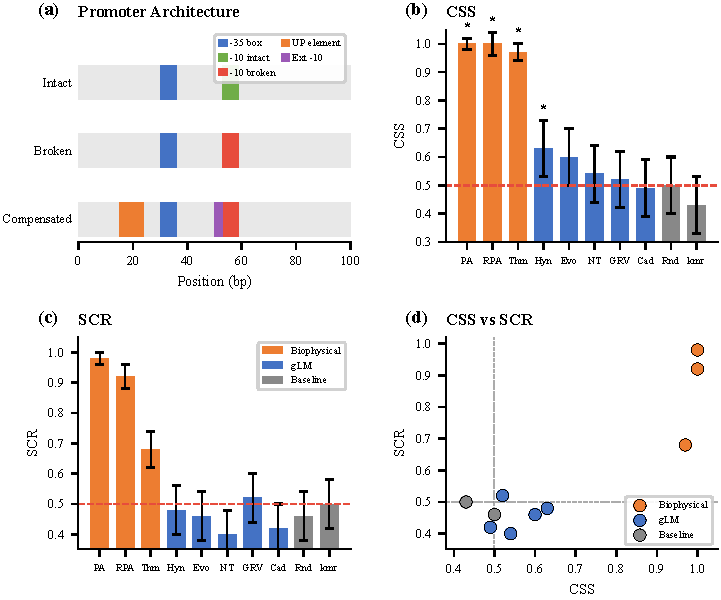
\includegraphics[width=\columnwidth]{figures/fig1_overview.pdf}
\vspace{-1em}
\caption{\textbf{MIT benchmark overview.} (a)~Promoter architecture.
(b)~CSS across models; asterisk indicates $p_{\text{FDR}}{<}0.05$.
(c)~SCR: all gLMs cluster near chance (0.5).
(d)~CSS vs.\ SCR: biophysical models (orange) occupy the upper-right
quadrant indicating epistemic validity; gLMs (blue) cluster along the
x-axis revealing overconfident misattribution.}
\label{fig:overview}
\end{figure}

\subsection{Primary Results}

\Cref{tab:main_results} presents the central finding.
After FDR correction, only HyenaDNA achieves significant CSS
($p_{\text{FDR}}{=}0.034$).
But the epistemic diagnosis lies in the SCR column: \emph{all} gLMs show
SCR near or below 0.5 (range: 0.40--0.52).
Not one model---across architectures ranging from 1.9M to 1B
parameters---distinguishes correctly positioned from scrambled
compensation.
All gLMs also show negative MES$_\text{syn}$, meaning they score broken
sequences \emph{higher} than intact ones, inverting biological reality.

The CSS/SCR dissociation is the definitive epistemic signature:
HyenaDNA appears sensitive to compensation (CSS $= 0.63$) while being at
chance on positional discrimination (SCR $= 0.48$).
The model has detected a real correlate---AT-richness---while encoding
nothing about \emph{why} it correlates with function.

\begin{table}[t]
\caption{MIT results. All gLMs show SCR near or below 0.5 regardless
         of architecture, revealing universal positional blindness.
         The CSS/SCR gap is the epistemic signature.}
\label{tab:main_results}
\vskip 0.05in
\centering
\small
\begin{tabular}{@{}lcccc@{}}
\toprule
Model & CSS & $p_{\text{FDR}}$ & SCR & MES$_\text{syn}$ \\
\midrule
\textbf{HyenaDNA} & \textbf{0.63} & \textbf{0.034} & 0.48 & $-$0.34 \\
Evo2-1B           & 0.60          & 0.090          & 0.46 & $-$0.03 \\
NT-500M           & 0.54          & 0.569          & 0.40 & $-$0.10 \\
GROVER            & 0.52          & 0.691          & 0.52 & $-$0.05 \\
Caduceus          & 0.49          & 0.772          & 0.42 & $-$0.40 \\
\midrule
Random            & 0.50          & ---            & 0.46 & $-$0.04 \\
k-mer             & 0.43          & ---            & 0.50 & $+$0.11 \\
\bottomrule
\end{tabular}
\vskip -0.05in
\end{table}

\subsection{Probing the Epistemic Failure}

We conduct four mechanistic experiments to characterize \emph{how} gLMs
fail epistemically, varying one causal factor at a time.

\subsubsection{AT Content: Spurious Confidence}

We vary background AT content from 30\% to 80\% while holding motif
identities constant (\Cref{tab:at_titration}).
Log-likelihood increases monotonically with AT content across all models
($r = 0.78$--$0.96$).
Compensated sequences (Class E) contain AT-rich UP elements
(${\sim}89\%$ AT) that locally elevate AT content;
this explains CSS $> 0.5$ in its entirety.
The model is not encoding \emph{why} the UP element helps---it encodes the
raw fact that AT-rich sequences score higher.
This is precisely overconfident misattribution: high confidence in a
spurious correlate.

\begin{table}[t]
\caption{AT content drives model predictions. Monotonic AT-LL
         correlation ($r{=}0.78$--$0.96$) across all architectures
         fully explains apparent compensation sensitivity.}
\label{tab:at_titration}
\vskip 0.05in
\centering
\small
\begin{tabular}{@{}lcc@{}}
\toprule
Model     & AT-LL Corr.   & Architecture \\
\midrule
Evo2-1B   & $r = 0.961$   & Autoregressive \\
Caduceus  & $r = 0.874$   & Bidir.\ SSM \\
HyenaDNA  & $r = 0.784$   & Autoregressive \\
\bottomrule
\end{tabular}
\vskip -0.05in
\end{table}

\subsubsection{Positional Inversion: Confident Misdirection}

We compare sequences placing the UP element at the correct position
(pos.\ 15, upstream of -35) vs.\ the wrong position (pos.\ 70, downstream
of -10).
Evo2-1B and Caduceus score the \emph{wrong position higher} than correct
($\Delta = {+}0.55$ and ${+}0.75$ respectively).
This is not mere uncertainty---it is confident misdirection: the models
are \emph{more confident} about the incorrect configuration.
Compositional effects (removing UP entirely: $\Delta \approx 1.5$--$3.7$)
dominate positional effects by 46-fold, confirming that position is
essentially invisible to these models.

\subsubsection{Spacing: Miscalibrated Preferences}

The biological optimum for -35/-10 spacing is $17{\pm}1$ bp
\citep{harley1987analysis}.
HyenaDNA's likelihood peaks at 14~bp, not 17~bp.
This is a calibrated-but-wrong preference: the model has learned
\emph{some} spacing sensitivity, but the epistemic content is wrong---its
confidence maximum does not align with biological function.

\subsubsection{Strand Blindness: Missing Causal Dimension}

Forward promoter sequences score \emph{lower} than reverse complement
variants (44\% accuracy; binomial $p = 0.24$ vs.\ 50\% chance baseline).
Strand orientation is a fundamental causal factor---the sequence is only
transcribed from the correct strand---yet all tested gLMs are effectively
strand-blind.
A model with epistemic intelligence about transcription would represent
which strand is functional; current gLMs encode no such information.

\begin{figure}[t]
\centering
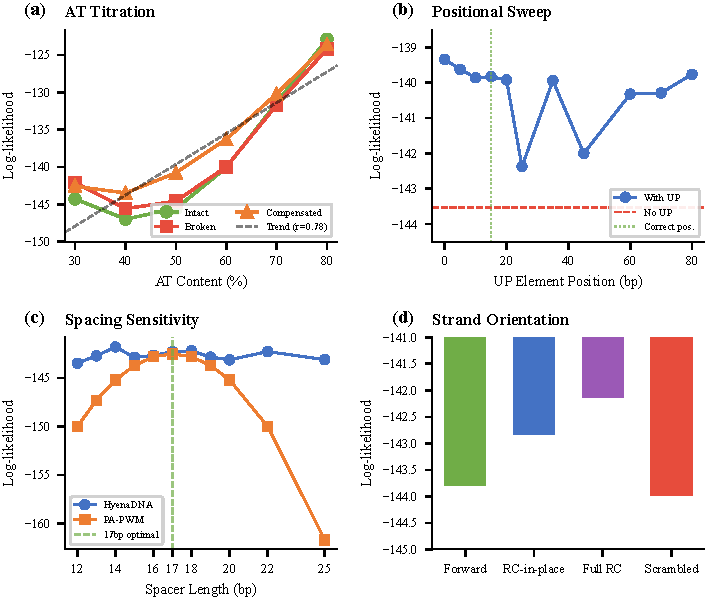
\includegraphics[width=\columnwidth]{figures/fig2_results.pdf}
\vspace{-1em}
\caption{\textbf{Four epistemic failure modes.} (a)~AT titration:
LL scales monotonically with AT composition ($r{=}0.78$).
(b)~Positional ablation: removing UP (compositional, $\Delta{\approx}3.7$)
dominates misplacing it (positional, $\Delta{\approx}0.5$) by $46\times$.
(c)~Spacing: HyenaDNA peaks at 14~bp vs.\ biological optimum 17~bp.
(d)~Strand: forward orientation scores lower than RC, inverting biology.}
\label{fig:probing}
\end{figure}

\subsection{Biophysical Baseline: Epistemic Intelligence is Achievable}

To establish that our benchmark is solvable, we evaluate position-aware
biophysical baselines (\Cref{tab:biophysical}).
\textbf{PA-PWM} scores motifs at expected positions with compensation
bonuses (${\sim}100$ parameters, CSS$=$1.00, SCR$=$0.98).
\textbf{RPA-PWM} uses \emph{no hardcoded positions}---only relative
biological constraints: 17$\pm$2 bp spacing, UP upstream of -35, extended
-10 adjacent to -10, strand consistency---yet achieves CSS$=$1.00,
SCR$=$0.92.

The ablation is decisive: removing positional encoding from PA-PWM
(PA-PWM-NoPos) yields CSS$=$0.63, SCR$=$0.56---precisely matching
HyenaDNA's profile.
This means HyenaDNA has effectively learned PA-PWM-NoPos:
it detects compensation elements but not their positions.
A 100-parameter model with the right epistemic structure outperforms
billion-parameter networks with the wrong one.

\begin{table}[t]
\caption{Biophysical models achieve both high CSS and high SCR,
         demonstrating that positional encoding is learnable.
         PA-PWM-NoPos ablation matches HyenaDNA exactly, showing gLMs
         have learned composition without position.}
\label{tab:biophysical}
\vskip 0.05in
\centering
\small
\begin{tabular}{@{}lccr@{}}
\toprule
Model             & CSS  & SCR  & Params \\
\midrule
PA-PWM            & 1.00 & 0.98 & $\sim$100 \\
RPA-PWM           & 1.00 & 0.92 & $\sim$100 \\
Thermodynamic     & 0.97 & 0.68 & $\sim$50  \\
\midrule
PA-PWM-NoPos      & 0.63 & 0.56 & $\sim$100 \\
\midrule
HyenaDNA          & 0.63 & 0.48 & 6.6M \\
Evo2-1B           & 0.60 & 0.46 & 1B   \\
Caduceus          & 0.49 & 0.42 & 1.9M \\
\bottomrule
\end{tabular}
\vskip -0.05in
\end{table}

%----------------------------------------------------------------------
\section{Discussion}
\label{sec:discussion}
%----------------------------------------------------------------------

\subsection{Scale Amplifies Epistemic Miscalibration}

The consistent failure pattern across five architectures establishes that
the epistemic failure is not model-specific but a fundamental property of
current gLM pretraining.
More troublingly, scale \emph{amplifies} rather than corrects it:
Evo2-1B (1B parameters) shows 23\% stronger AT-correlation
($r{=}0.96$) than HyenaDNA (6.6M parameters, $r{=}0.78$).
Larger models fit the AT-richness heuristic more precisely.
This is consistent with the underspecification hypothesis
\citep{d2020underspecification}: when multiple functions are compatible
with training data, larger models converge more confidently on whichever
solution minimizes training loss, even if that solution is mechanistically
wrong.
Sequence likelihood pretraining on genomic data rewards AT-richness
recognition at every scale; positional constraint encoding is never
directly incentivized.

\begin{figure}[t]
\centering
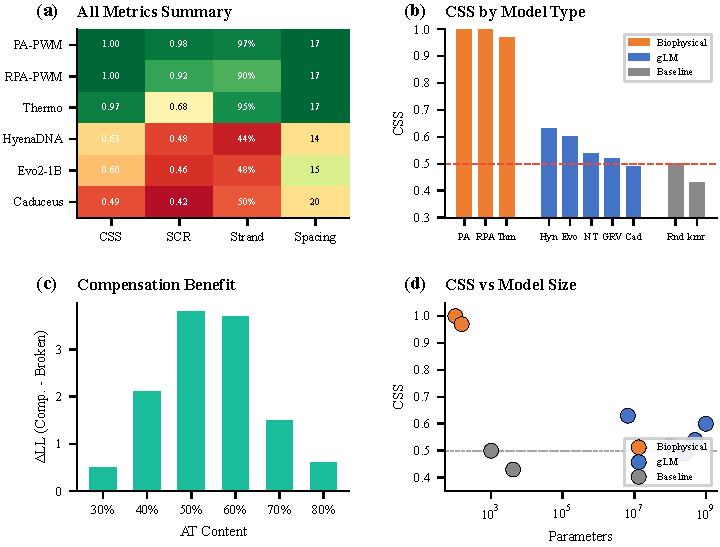
\includegraphics[width=\columnwidth]{figures/fig4_summary.pdf}
\vspace{-1em}
\caption{\textbf{Universal epistemic failure.} All four failure modes---AT
confound, positional inversion, spacing miscalibration, strand
blindness---are consistent across architectures.
Scale amplifies rather than corrects each failure.}
\label{fig:summary}
\end{figure}

\subsection{Connections to the EIML Program}

Our results bear directly on several open questions in epistemic
intelligence for machine learning:

\textbf{Confidence vs.\ competence.}
The CSS/SCR dissociation shows that high apparent competence
(CSS $> 0.5$, significant FDR-corrected $p$-values) can coexist with
fundamentally miscalibrated representations.
Standard calibration metrics---measuring whether predicted probabilities
match empirical frequencies---would not detect this failure.
Models are not overconfident about their \emph{predictions}; they are
overconfident about their \emph{representations of causation}.
This is a new kind of epistemic failure that existing calibration
frameworks do not measure.

\textbf{Representation uncertainty vs.\ predictive uncertainty.}
Current uncertainty quantification (UQ) methods focus on predictive
uncertainty: how confident should the model be about a specific
prediction \citep{guo2017calibration,ovadia2019can}?
Our results suggest a complementary need for \emph{representation
uncertainty}: how confident should the model be that it has identified
the correct causal factors?
A model with high representation uncertainty would appropriately hedge
when asked to score a compensated sequence, recognizing that its
AT-richness heuristic may not be the true signal.
Current gLMs show no such hedging.

\textbf{Inductive biases as epistemic priors.}
PA-PWM's success with ${\sim}100$ parameters demonstrates that the
bottleneck is inductive biases, not capacity.
A model that explicitly represents position-dependent scoring has the
right epistemic prior; a model that encodes raw sequence statistics does
not.
This suggests that epistemic intelligence in biology may require
architectural innovations that build in causal structure:
position-aware attention mechanisms, contrastive objectives that
discriminate scrambled from correctly placed elements during training,
or hybrid architectures combining neural encoders with differentiable
biophysical modules \citep{avsec2021bpnet,alipanahi2015predicting}.

\textbf{Diagnosing misattribution in other domains.}
MIT provides a reusable template for constructing epistemic probes
wherever a causal mechanism is known:
(1)~identify a biological case where composition and position are
dissociable with matched controls; (2)~define CSS-type and SCR-type
metrics that jointly test presence and position sensitivity;
(3)~measure the CSS/SCR dissociation as the epistemic failure signature.
This methodology could apply to protein structure prediction (where
contact maps have known positional logic), regulatory network inference,
or RNA secondary structure prediction---any domain with ground-truth
mechanistic constraints.

\subsection{Towards Epistemic Calibration}

Three concrete directions follow from our analysis.
First, \textbf{contrastive pretraining objectives} that require models to
assign lower likelihood to scrambled vs.\ correctly positioned elements
directly incentivize positional encoding.
Second, \textbf{position-aware architectures}---attention biases encoding
known spacing distributions, or convolutions with biologically motivated
receptive fields---impose the right inductive prior.
Third, \textbf{causal probing} during model development, using benchmarks
like MIT to verify that learned representations align with known
mechanisms before deployment in clinical or synthetic biology
applications.

%----------------------------------------------------------------------
\section{Related Work}
%----------------------------------------------------------------------

\textbf{Genomic language models.}
gLMs have evolved from k-mer methods \citep{lee2011discriminative} to
large transformers \citep{ji2021dnabert,dalla2023nucleotide,zhou2023dnabert2}
and efficient state-space architectures
\citep{nguyen2023hyenadna,schiff2024caduceus}.
Evaluation has focused on downstream task performance; whether these
models learn mechanistic principles has received limited attention.

\textbf{Mechanistic interpretability.}
In NLP, probing methods localize syntax representations
\citep{hewitt2019structural} and factual knowledge
\citep{meng2022locating}.
In genomics, post-hoc motif extraction from attention weights
\citep{novakovsky2023obtaining} asks \emph{what} models attend to but
not whether attention corresponds to causal function.
Our approach---systematically varying causal factors with matched
controls---is closer in spirit to causal abstraction
\citep{geiger2021causal} and interchange interventions
\citep{meng2022locating}.

\textbf{Calibration and epistemic uncertainty.}
Calibration research \citep{guo2017calibration} and ensemble methods
\citep{lakshminarayanan2017simple} address predictive uncertainty but
not representation uncertainty.
\citet{d2020underspecification} show that models trained on the same
data can converge to functionally different solutions---our results
suggest gLMs converge to the AT-richness solution, not the mechanistic
one.

\textbf{Promoter biology.}
Quantitative $\sigma^{70}$ models \citep{brewster2012lac,kinney2010using}
and well-characterized compensation mechanisms
\citep{ross1993third,barne1997region} provide ground truth that enables
rigorous evaluation of mechanistic encoding.

%----------------------------------------------------------------------
\section{Conclusion}
%----------------------------------------------------------------------

MIT reveals that genomic language models exhibit a characteristic form
of epistemic failure: overconfident misattribution.
They correctly detect AT-richness---a real correlate of promoter
strength---while completely failing to encode the positional constraints
that determine whether AT-richness is functionally relevant.
Across five architectures from 1.9M to 1B parameters, no model
distinguishes correctly positioned from scrambled regulatory elements.
That scale amplifies rather than corrects this failure, and that a
100-parameter model with proper epistemic structure outperforms all
gLMs, establishes a clear diagnosis: the bottleneck is inductive biases
and pretraining objectives, not capacity.

MIT provides a reusable diagnostic for measuring epistemic intelligence
in gLM development.
More broadly, the CSS/SCR framework---measuring both what models detect
and whether they know \emph{where} it matters---offers a template for
epistemic probing in any domain with known causal structure.
We release all code, data, and inference scripts to support this
program.

\subsubsection*{Reproducibility}
All code, data, and model inference scripts available at
\url{https://github.com/bryanc5864/MechanisticInvarianceTest}.
Results are fully reproducible with fixed random seed (42) via a single
command.

\bibliography{references}
\bibliographystyle{icml2026}

\end{document}
